\section{Methodology}

\begin{figure*}[t]
  \centering

   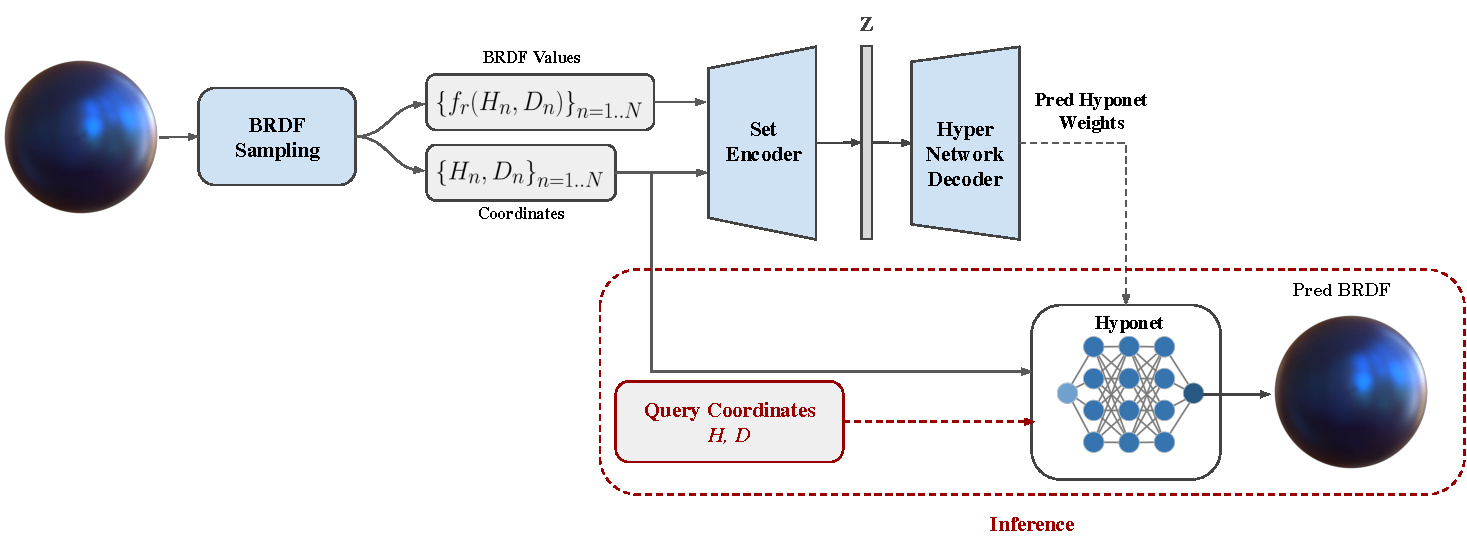
\includegraphics[width=\linewidth]{Chapters/hyperbrdf-figs/MainFig_13_11.pdf}
   \caption{During training, the set encoder and hypernetwork decoder are trained on a set of materials to predict the weights of hyponet (MLP) so that it can reconstruct the training set. The BRDF data is provided as a set of BRDF coordinates, $H_n,D_n$, and the corresponding reflectance values $f_r(H_n,D_n)$. To reconstruct a new material from a small set of BRDF reflectance samples, the trained set encoder and hypernetwork decoder are used to predict the weights of hyponet for the unknown material. Once those weights are known, we can query BRDF at any coordinates and for any new materials, conditioned on the embedding of their sampled BRDF values.}
   \label{fig:mainfig} \end{figure*}

Based on the observation that recent work misses a generalised and adaptable \gls{BRDF} representation, I introduce a novel representation for measured \gls{BRDF}s that learns compact embeddings of the \gls{BRDF}s with a hypernetwork model.

\subsection{Pre-processing}\label{sec:pre-proc}

Measured \gls{BRDF}s usually contain high dynamic range (\gls{HDR}) data, including arbitrarily high values, especially for the specular components. Hence, I pre-process the \gls{BRDF} data by applying a Log Relative Mapping~\cite{nielsen2015optimal} of the form:
\begin{equation}
  \rho' = \ln{\left(\frac{\rho + \epsilon}{\rho_{ref} + \epsilon} +1\right)}
  \label{eq:preprocess}
\end{equation}
where $\rho$ refers to the \gls{BRDF} values, $\epsilon = 0.002$ is a small constant value to avoid zero-division, and $\rho_{ref}$ is a reference \gls{BRDF} value for relative mapping. The reference \gls{BRDF} value is chosen to be the median value for each angle over the entire dataset.


We also observe that input parameterisation has a strong impact on the reconstruction quality since it guides the neural network model to learn different aspects of the reflectance function. Therefore, similar to NBRDF~\cite{sztrajman2021neural}, I express the \gls{BRDF}s as functions of the Cartesian vectors $H$ and $D$ in the Rusinkiewicz parameterisation \cite{rusinkiewicz1998new},
\textit{i.e.}, $\rho=f_r(H, D)$, where $H, D \in S^2$ indirectly encode the information about the incident and outgoing light directions.

Importantly, in this parameterization the directions of specular reflection have a single fixed representation as $H=(0,0,1)$, which provides an easier pattern for the network to learn than the traditional $\omega_i, \omega_o$ encoding.


\subsection{Hypernetwork}
\label{sec:hypernet}

Figure~\ref{fig:mainfig} shows the diagram of the hypernetwork model~\cite{sitzmann2020siren} for \gls{BRDF} representation, with three main components: 1) a set encoder that generates compact latent representations $Z$ of \gls{BRDF}s based on an arbitrary number of directional samples, 2) a hypernetwork decoder that decodes the latent to estimate the parameters of a neural field,
and 3) a neural field controlled by the decoder that represents the \gls{BRDF}s of the material, which we refer to as a hyponet, following the convention of prior work~\cite{sitzmann2020metasdf}.


\subsubsection{Set encoder} %add number of layers

The set encoder takes as input an arbitrary set of samples, $n=1..N$, taken from a \gls{BRDF} measurement. Each measurement consists of directional coordinates ${H_n, D_n}$, given in the Rusinkiewicz parameterisation~\cite{rusinkiewicz1998new}, and their corresponding \gls{BRDF} values $f_r(H_n,D_n)$. The set encoder is composed of four fully-connected layers with two hidden layers of feature size 128 for each. The input is the concatenation of \gls{BRDF} values $(N, 3)$ and coordinates $(N, 6)$. The activation function applied after each layer is \gls{ReLU}. Each sample is encoded into a 40-dimensional embedding, and the sample set is reduced to a single embedding by applying a symmetric operation (averaging).
% \FZ{Permutation invariant operations are common in point set networks. Consider referring to the literature to motivate our design over alternatives.}
The use of a set encoder, which is commonly adopted in point set networks \cite{zaheer2017deepsets}, ensures permutation invariance and provides a high degree of flexibility in terms of the input, enabling the encoding of \gls{BRDF}s with an arbitrary number of data-points, irregularly sampled, and in no pre-defined order.


\subsubsection{Hypernetwork decoder and hyponet} %add number of layers and type
The hypernetwork decoder converts the embeddings from the set encoder into the weights of the hyponet that represents the \gls{BRDF}s of a single material. The hypernetwork decoder is composed of 10 blocks of a fully-connected neural network with three layers. Each block outputs the corresponding weights and biases of hyponet. The hyponet consists of five fully-connected layers with input layer of size six for coordinates, three hidden layers of size 60 for each, output layer of size three for \gls{BRDF} values. The neural representation of materials, hyponet, follows the structure of NBRDF~\cite{sztrajman2021neural}, but replaces the exponential activation (\gls{ELU}) in the last layer with a \gls{ReLU} activation due to \gls{BRDF} properties ($\rho \ge 0$). This network provides a continuous representation of a \gls{BRDF}, and has been shown to provide state-of-the-art reconstructions of measured \gls{BRDF}s, with performances competitive with the fastest analytic \gls{BRDF} models.


\subsection{Training}
\label{sec:traindet}


I train the hypernetwork by optimizing the following loss, which consists of a reconstruction term $\mathcal{L}_\text{rec}$ and two regularization terms $\mathcal{L}_\text{weights}$ and $\mathcal{L}_\text{latent}$ for the hyponet weights $w$ and the latent embeddings $z$ ~\cite{ha2017hypernetworks}:
\begin{equation}
    \mathcal{L} = \mathcal{L}_\text{rec} +
              \lambda_1 \underbrace{\frac{1}{W} \sum_{j=1}^W w^2_j}_{\mathcal{L}_\text{weights}} +
              \lambda_2 \underbrace{\frac{1}{Z} \sum_{k=1}^Z z^2_k}_{\mathcal{L}_\text{latent}}
    \label{eq:loss}
\end{equation}

The reconstruction loss is defined as the mean squared error between the cosine weighted predicted and ground-truth \gls{BRDF} values:

\begin{equation}
    \mathcal{L}_{\text{rec}} = \sum_{n=1}^{N}\sum_{m=1}^{M}\frac{\left|\left|\rho^{\text{pred}}_{n, m} \cos{\theta_{n, m}} - \rho^{\text{true}}_{n, m} \cos{\theta_{n, m}}\right|\right|_{2}}{NM}
    \label{eq:Lrec}
\end{equation}

where $\rho^{\text{pred}}_{n, m}$ and $\rho^{\text{true}}_{n, m}$ indicate the predicted and ground truth \gls{BRDF} values of the $n$-th sample of the $m$-th material, both processed as described in Eqn \ref{eq:preprocess}, and $\theta$ measures the angle between the incident ray and the surface normal. The cosine term weighs \gls{BRDF}s based on the assumption of uniform incoming radiance and leads to more visually accurate results \cite{ngan2005experimental}.


I train the network for 80 epochs with 1,458,000 samples per material. It takes around 15 minutes with an NVIDIA A100 80GB GPU support. 


\paragraph{Inference:}
When inferring the reflectance values, HyperBRDF first estimates hyponet weights from sparse samples of a test material, which takes around 0.01 seconds without GPU. Later, I feed query coordinates to the hyponet to predict the \gls{BRDF} values of the material. With the conversion of the predicted \gls{BRDF} into a renderable format, this process takes around 9 seconds without GPU. The continuous representation of \gls{BRDF}s with the hyponet offers a nonlinear built-in interpolation and, hence, accurately reconstruct unseen materials from even a few samples.